\subsection{Anti-serialization}
In \cref{fig:trivial-example} we see that some items will have to move through modules, where no work is performed on them. This will often happen if we have a line of modules, where more than one type of item is to be produced. We would like to describe a rule, which breaks the serial connection of a line of modules. It should be able to make an off branch from a line, moving into the new branch a sequence of modules, which are only used by one type of item. We call this operation an anti-serialization on a line. Performing several anti-serializations across a line, decreases the amount of unneeded modules which each item need to pass through. This should eventually increase the total throughput. In this subsection we describe different transformation rules, which are needed to perform anti-serialization upon a line.

\subsubsection{Branching between common modules}
Let us say that we want to branch out a specific recipe $r$ from a line $\gamma$. Here we first define a special set on $r$, $\bar{r}$, which contains all types of work which are not unique to $r$:
\[\bar{r} = \bigcup_{r' \in R}r', \texttt{ if } r' \neq r\]

Next we need to define what we would like to call common modules. These are module in $\gamma$, which $r$ needs to use along with at least some other recipe. These are important to identify, as they may not be branched out, as that would make the inaccessible to the other recipes that might need it.  Given $r$ and $\gamma$ we define the set of common modules $K_{\gamma ,r}$ as follows:

\[K_{\gamma ,r} = \{m \in \gamma | \gamma \in \Gamma \land \exists \rho \in m.aW,\, \{\rho\} \subseteq r \land \{\rho\} \subseteq \bar{r} \land r \in R\}\]

From this set we can then define $\alpha_{\gamma ,r}$, which is the set of modules in $\gamma$ which are not used by $r$: 

\[\alpha_{\gamma ,r}  = \{m \in \gamma | \gamma \in \Gamma \land \forall \rho \in m.aW,\, \{\rho\} \nsubseteq r \land r \in R\}\]

Along with $\beta_{\gamma ,r}$, which is the set of modules in $\gamma$ used only by $r$:

\[\beta_{\gamma ,r}  = \{m \in \gamma | \gamma \in \Gamma \land \forall \rho \in m.aW,\, \{\rho\} \subseteq r \land \{\rho\} \nsubseteq \bar{r} \land r \in R\}\]

We now want to define a set of all neighbours of common modules in line $\gamma$. Two modules $m_1$ and $m_2$ are said to be neighbours within a set if $m_1 <_k m_2$ holds true. The relation does this if $m_1$ $\prec$ $m_2$ evaluates to true, while $m_1 \prec m_i \land m_i \prec m_2, m_i \in K_{\gamma ,r}$ is not true. Having set up this relation, we can define the set of all common module neighbours $KP_{\gamma ,r}$ as:
 
\[KP_{\gamma ,r} = \{(s, e)| {s, e} \in K_{\gamma ,r} \times K_{\gamma ,r} \land s <_k  e\}\]


We also define a set of all modules in between two other modules, $s$ and $e$, in the line $\gamma$. 

\[M_{s,e} = \{m | m \in \gamma \land \gamma \in \Gamma \land s \prec m \land m \prec e\}\]

We can now define the set of all modules appearing between $s$ and $e$, which are not used to work $r$ $A_{s,e}$ as follows: 

\[A_{s,e} = \{m |m \in M_{s,e} \land m \in \alpha\}\]

Similarly we can define the set $B_{s,e}$, which contains all modules that appear between $s$ and $e$ which are only used to perform work on $r$

\[B_{s,e} = \{m |m \in M_{s,e} \land m \in \beta\}\]

Having now defined our sets, we will set up the rules describing how we may branch out modules to work on individual recipes. These rules will be described informally using our own graphical notation. The graphical notation works as follows. Square boxes represent modules. Boxes with rounded corners represent a set of modules totally ordered on $\prec$. The modules within the box are connected left to right according to their order. Connections going to the box connect to the first element of the order and connections leaving from the box come from the last module. If a set box only contains "..." it means that some set of modules may be here, but there is no need to consider what it contains. 

Now imagine the situation in \cref{fig:asbase}. Here we have specific $s$ and $e$ modules chosen on a line $\gamma$ and we have chosen to branch out a specific recipe $r$. Between the two modules we may have $M_{s,e}$ placed. From this we can calculate $A_{s,e}$ and $B_{s,e}$ as described before. If $B_{s,e} = \emptyset$ then we may branch out some modules only used to work on $r$. 

\begin{figure}[h]
\centering
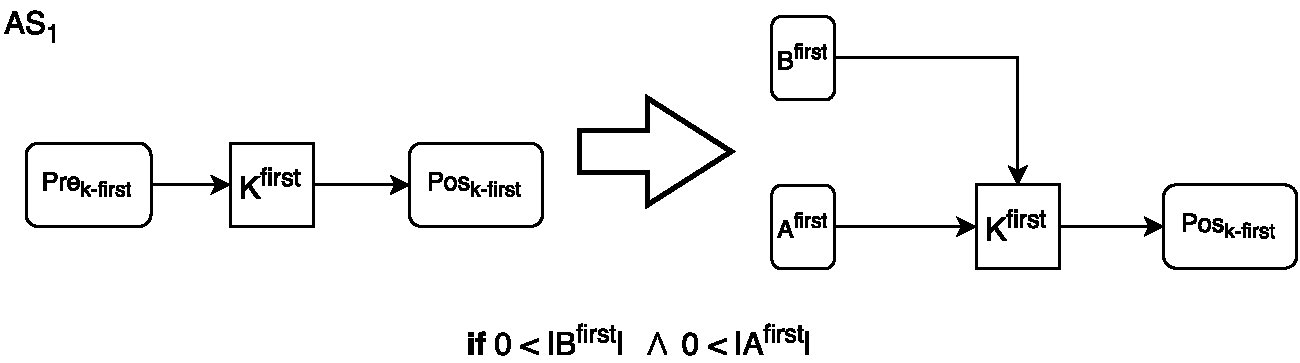
\includegraphics[width=\textwidth]{as1.pdf}
\caption{A base configuration where we may want to branch out recipe $r$ from line $\gamma$}
\label{fig:asbase}
\end{figure}

If $|A_{s,e}| = |B_{s,e}| + 2$ , then we can branch out as shown in the top of \cref{fig:astrans}. Here we simply remove $|B_{s,e}|$ from the rest of $M_{s,e}$ leaving us with in its place $A_{s,e}$. The module $s$ is then connected upwards to the first element of $|B_{s,e}|$. The last element of $|B_{s,e}|$ is then connected to $e$. This transformation also entails that all of  $|B_{s,e}|$ is removed from $\gamma$ and that a new line containing $|B_{s,e}|$ is added to $\Gamma$. For each of the transformations presented in this subsection we alter $\gamma$ and add to $\Gamma$ the new branch which is created.  Notice that the modules beneath the new line are marked as red. This means that the shadow variable in the module tuples on the old line have been set to true. This is used in order to handle transformation conflicts as described later in \cref{ssec:tc}.

In the middle of \cref{fig:astrans} we describe the case where $A_{s,e}| > |B_{s,e}| + 2$. The difference between the cardinality of these two sets is called i.  In this case we can not physically connect the last element of $|B_{s,e}|$ downwards to $e$. We get around this issue by appending the new line with i new transport modules. These are modules which can not perform any work and are only used to transport recipes. The last of these transporters is then connected downwards to $e$. The new line added to $\Gamma$ consists of the modules in $|B_{s,e}|$ ordered behind the new transport modules as depicted in the figure. 

The last case, shown in the bottom of \cref{fig:astrans} is similar to the previous one, but instead $A_{s,e}| < |B_{s,e}| + 2$. In this case we append the original line with transporters instead. This requires an update of $\gamma$ to include these new transporters, while the new line added to $\Gamma$ is again just $|B_{s,e}|$. 

\begin{figure}[h]
\centering
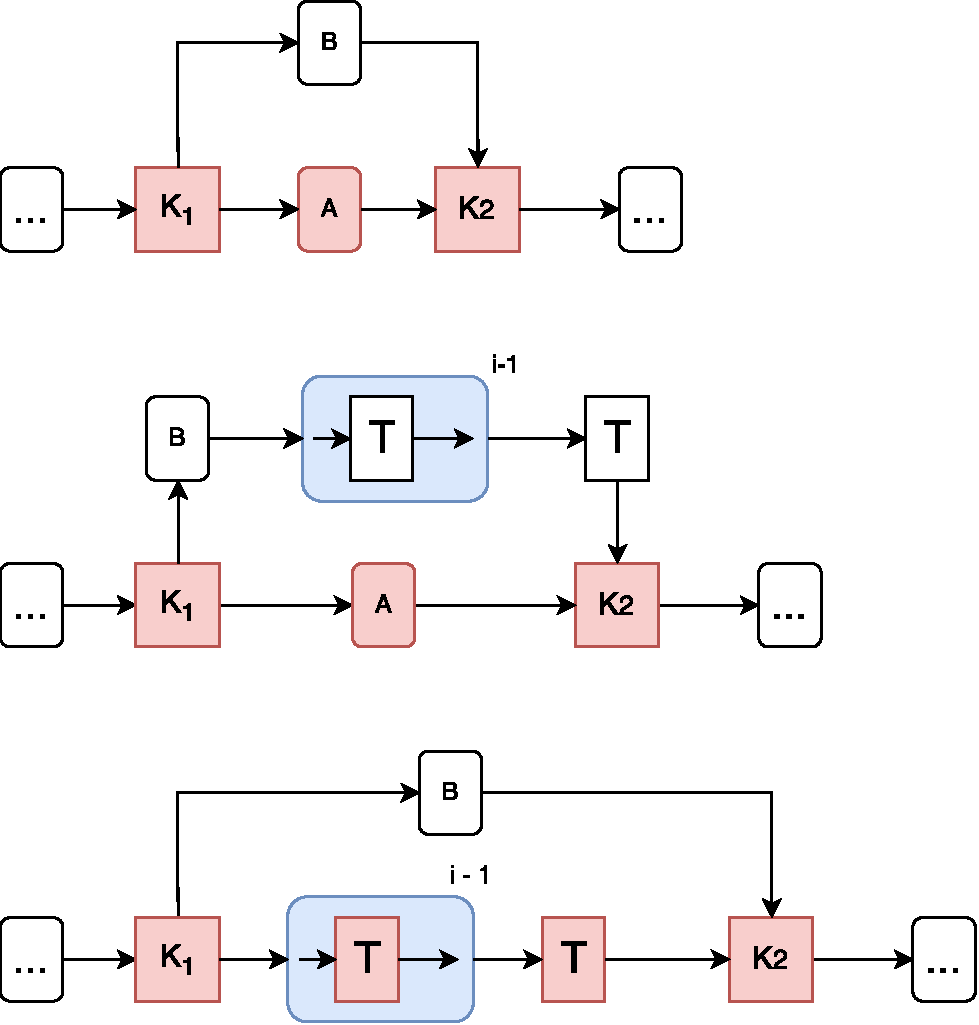
\includegraphics[width=\textwidth]{as2.pdf}
\caption{3 different configurations to which we may go from \cref{fig:asbase}. Top: Case when $A_{s,e}| = |B_{s,e}| + 2$. Middle: Case when $A_{s,e}| > |B_{s,e}| + 2$. Bottom: Case when $A_{s,e}| < |B_{s,e}| + 2$ }
\label{fig:astrans}
\end{figure}

In the rest of this sub-section we will describe two special cases known as branch in and branch out. 

\subsubsection{Early Branch In}\label{sssec:bi}
It may be that we have modules that precede the first module of $K_{\gamma ,r}$, known as $K_{first}$. We define a new operand to get all modules appearing before a module $s$ in its line:

\[Pre_{s} = \{m | m \in \gamma \land \gamma \in \Gamma \land m \prec s\}\]

Using this with $K_{first}$, we get the set of modules preceding $K_{first}$ known as $Pre_{K_{first}}$. We can then define the set $B_{first}$, containing modules used only by $r$ in $Pre_{K_{first}}$ as:

\[ B_{first} = \{m | m \in \beta_{\gamma ,r}  \land m \in Pre_{K_{first}} \} \]

Similarly the set of all modules preceding $K_{first}$, which do not exclusively work on $r$ as: 

\[ A_{first} = \{m | m \in \alpha_{\gamma ,r}  \land m \in Pre_{K_{first}} \} \]

With this in place we present the transformation rule in \cref{fig:asbranchin}. This describes how we in the above case are allowed to remove $B_{first}$ from the line $\gamma$ leaving  $A_{first}$. We then connect its last module to $K_{first}$. The new line which is added to $\Gamma$ is then $B_{first}$. This type of branch allows us to start $r$ away from other items.   


\begin{figure}[h]
\centering
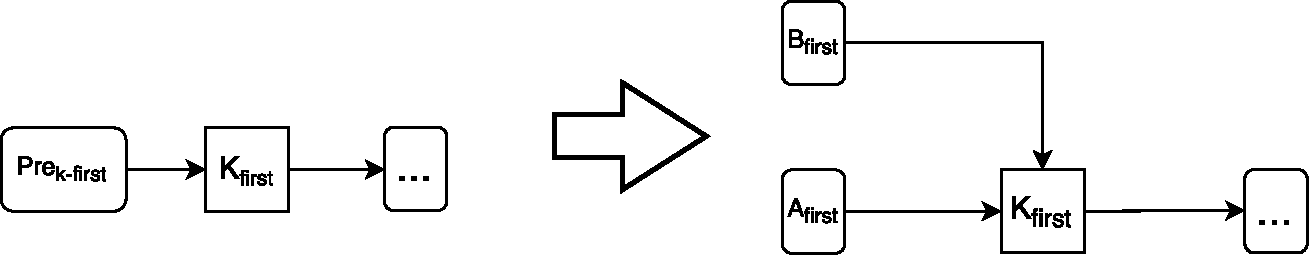
\includegraphics[width=\textwidth]{as4.pdf}
\caption{The case where modules precede the first module in $K_{\gamma ,r}$}
\label{fig:asbranchin}
\end{figure}

\subsubsection{Final Branch Out}
We have a similar case to \cref{sssec:bi}, where the last element in $K_{\gamma ,r}$, known as $K_{last}$, is proceeded by a set of modules. To get the modules proceeding $K_{last}$ we define the operand $Pro_{e}$ as follows:

\[Pro_{e} = \{m | m \in \gamma \land \gamma \in \Gamma \land e \prec  m \}\]

Using this on $K_{last}$ gives us $Pro_{K_{last}}$. The set containing all modules proceeding $K_{last}$, which exclusively work on $r$, is known as $B_{last}$ and is defined as:

\[B_{last} = \{m | m \in \beta_{\gamma ,r}  \land m \in Pro_{K_{last}} \}\]

The set of all modules proceeding $K_{last}$, which do not exclusively work on $r$, $A_{last}$ is given by:

\[ A_{last} = \{m | m \in \alpha_{\gamma ,r}  \land m \in Pro_{K_{last}} \} \]

Having set up this we present the final transformation rule for this type of branching in \cref{fig:asbranchout}. Here we see that in the described case we may remove $B_{last}$ from the line $\gamma$ leaving  $A_{last}$. $K_{last}$ is then connected to the first module of $B_{last}$. The new line added to $\Gamma$ is $B_{last}$. This transformation allows us to branch out $r$ when there is no need for it to stick with the old line never to return.


\begin{figure}[h]
\centering
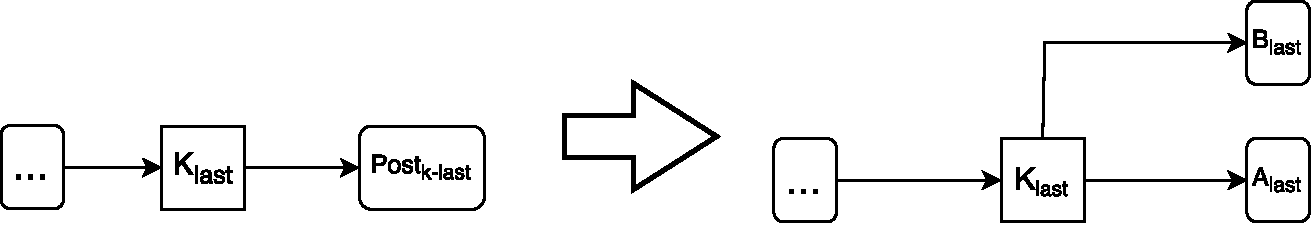
\includegraphics[width=\textwidth]{as3.pdf}
\caption{The case where modules proceed the last module in $K_{\gamma ,r}$}
\label{fig:asbranchout}
\end{figure}

\subsubsection{Restricting branches}
For the previous transformation rules, we have imagined that no other branch has been made from our line to any side. Yet, this will not always be the case. To be flexible enough to produce configurations with high throughput, we need to handle this. We go more in depth with how to enforce some general physical rules in \cref{ssec:conflicts}, but here we will tackle one unique to anti-serialization.

On the top part of \cref{fig:shadowexample}, we see that we have already made a branch from $s1$ to $e1$, which results in the modules on the old being shadowed. Being shadowed means that if we remove the module and just reconnect the old line as usual, then the branch becomes too long to connect back to its old line. The line needs to connect back to its designated point on the old line as the module located here is a common module. It performs work on the recipe $r$ otherwise worked on by the new line and should therefore not be bypassed.  To get around this we, as shown in \cref{fig:shadowexample}, alter our anti-serialization transformation in this case to replace a shadowed module with a transport module, as not to skew the two previous lines away from each other. The example shows this done for a single module, but it may be done regardless of the amount of shadowed modules which we remove.

We may however not do this if the shadowed module is also a module where a branch either connects from or to. This means that the module is common and is used by the branch. Removing it would keep us from producing that branch's specific recipe. Therefore we never allow for these modules to be removed, even if this means that we can not perform certain anti-serializations.

\begin{figure}[h]
\centering
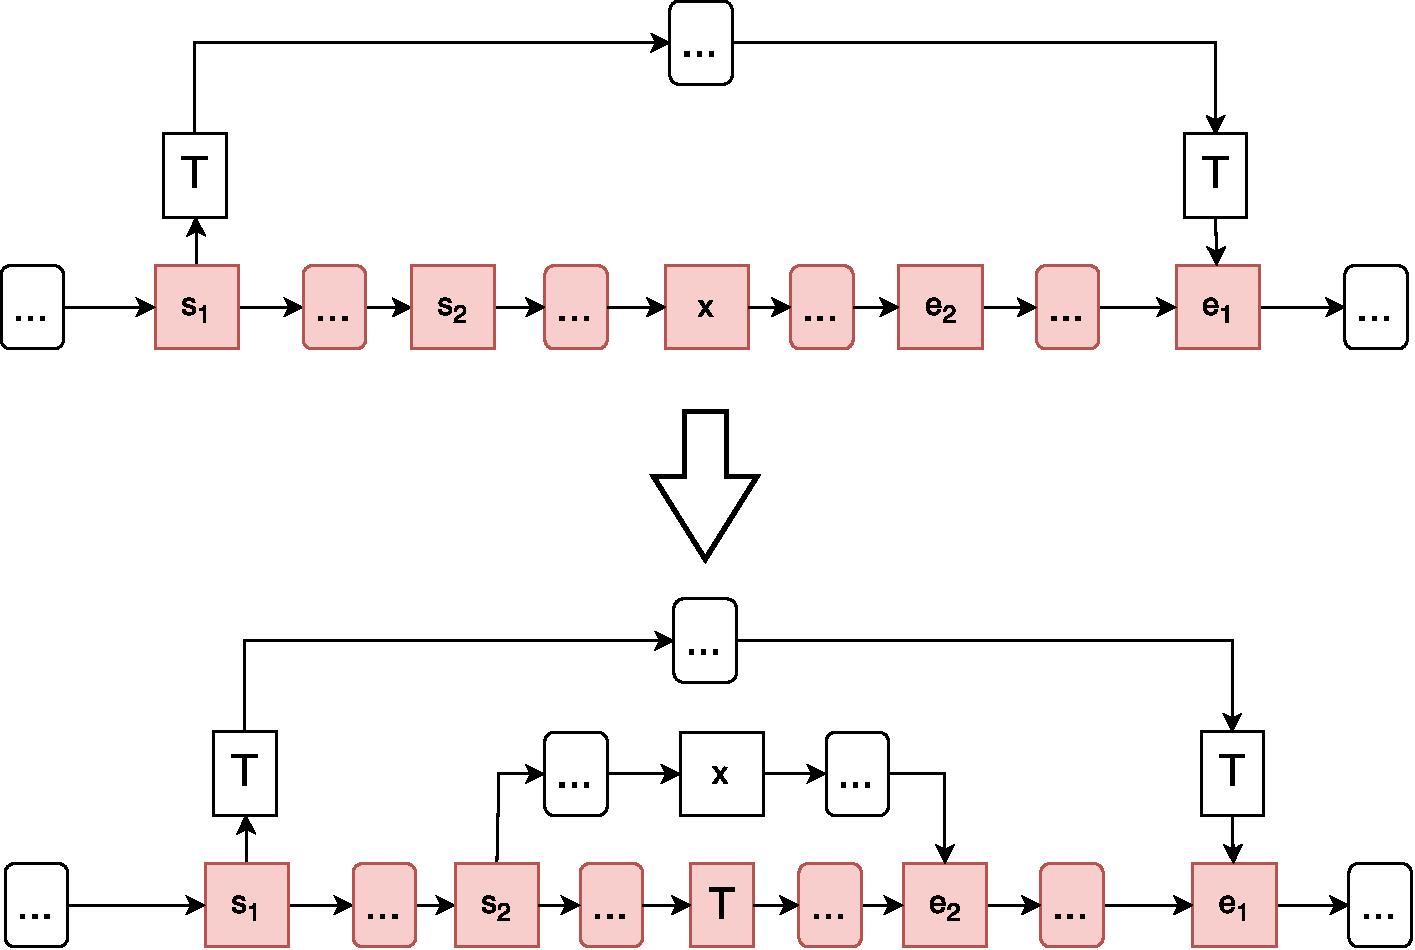
\includegraphics[width=\textwidth]{as5.pdf}
\caption{Transformation that handles the case where an anti-serialization removes a shadowed module}
\label{fig:shadowexample}
\end{figure}

